\documentclass{article}

\usepackage{mhchem}
\usepackage{siunitx}
\usepackage{graphicx}
\usepackage{caption}

\newcommand{\cc}{$\text{cm}^{3}$}
\newcommand{\circa}{\emph{circa }}

\title{Experiment 3 --- Synthesis and analysis of \ce{[Mo(CO)4(PPh3)2]}}
\date{24/11/2020}
\author{Samuel J. Frost -- pcysf6}

\begin{document}

\maketitle

\section*{Synthesis}
\subsection*{Part 1 --- Synthesis of \ce{[Mo(CO)4(morpholine)2]}}
Using oven dried equipment and under an atmosphere of dinitrogen \ce{[Mo(CO)6]}, (0.80 g), dry morpholine (9.00 \cc),
and dry heptane (20.0 \cc) were heated under reflux. The \ce{[Mo(CO)6]} dissolved to give a pale yellow solution.
After \circa 40 minutes the solution turned dull and then \circa 50 minutes yellow precipitate started to form.
After \circa 60 minutes precipitate ceased to form. The hot mixture was filtered via vacuum and washed 
with dry heptane (20 \cc). The yellow product was dried. (1.04 g, 89 \%)

\subsection*{Part 2 --- Synthesis of \ce{[Mo(CO)4(PPh3)2]}}
With the same setup as in Part 1 \ce{[Mo(CO)4(morpholine)2]} (0.62 g), triphenylphosphine (1.00 g) and 
dry dichloromethane (30.0 \cc) were heated to reflux for \circa 15 minutes. The solution was cooled to room temperature
and then filted under gravity. The solvent was removed under reduced pressure (until \circa 8 \cc) and methanol added (15 \cc).
The solution was cooled in an ice bath and the yellow crytals collected and dried via vacuum filtration. (0.60 g, 51 \%)

\newpage
\section*{Analysis}
The IR spectrum of \ce{[Mo(CO)4(PPh3)2]} in a solution of DCM was collected.

\begin{figure}[hp]
    \centering
    \captionsetup{justification=centering}
    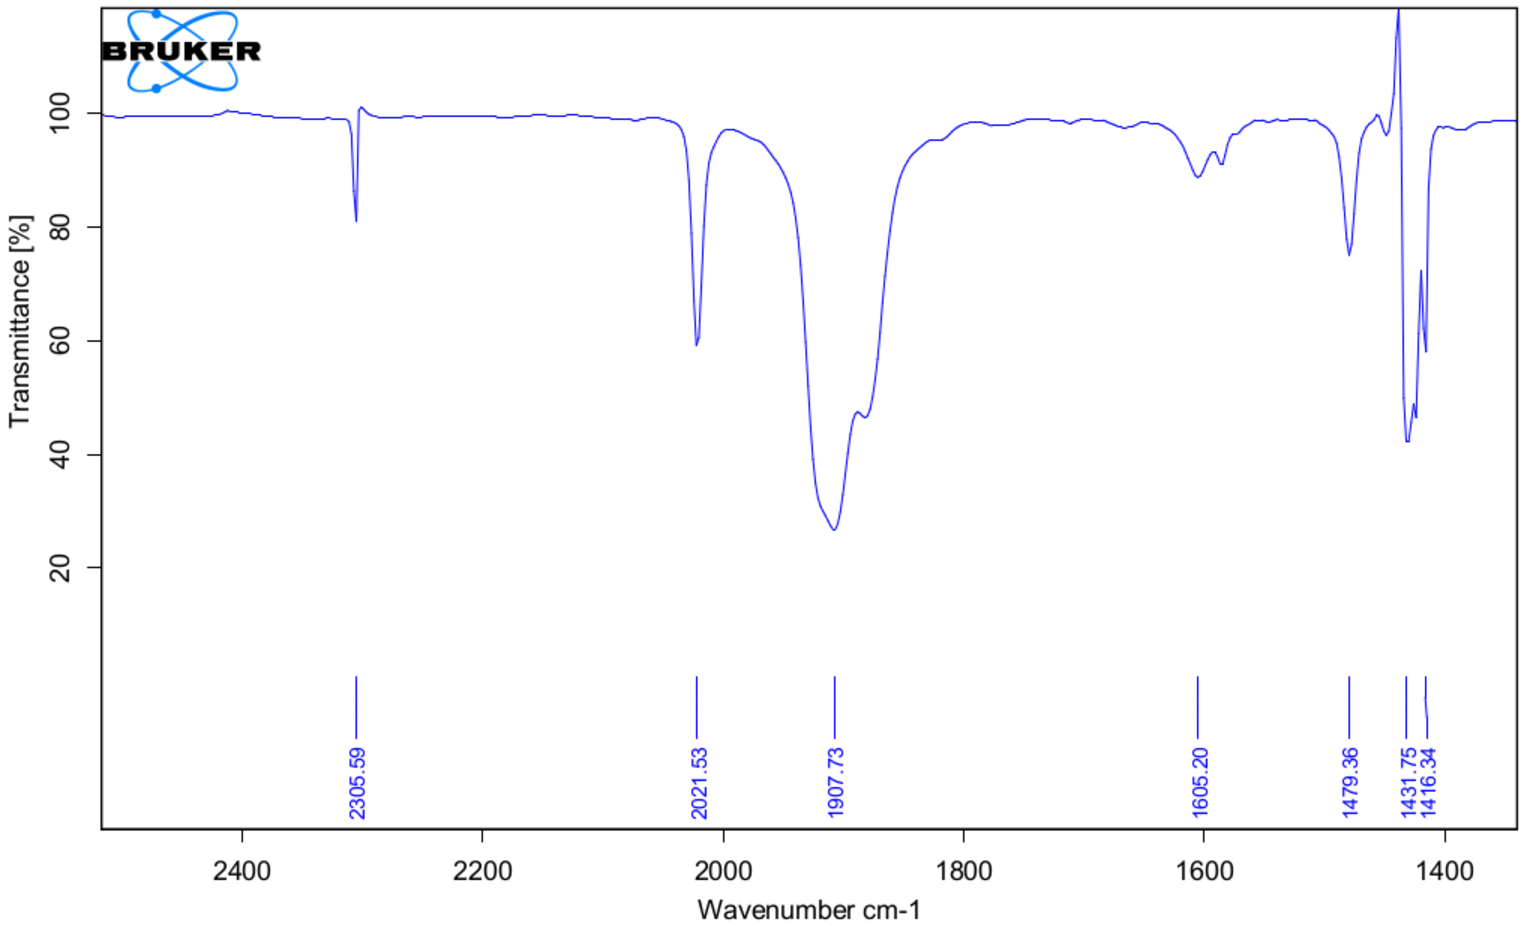
\includegraphics[width=13cm]{sam3.pdf}
    \caption{IR spectrum of \ce{[Mo(CO)4(PPh3)2]}}
\end{figure}


\end{document}